\documentclass[../main.tex]{subfiles}
\graphicspath{{\subfix{../../images/}}}
\begin{document}

\chapter{Experimental Methods}\label{chap:methods}

\bigskip
\begin{quote}
    \emph{We have some idea as to the intricate design of the puppet and the puppet strings, but we lack insight into the mind of the puppeteer\cite{bizziHardScientificQuest2015}.}\\
    \raggedleft{--- Emilio Bizzi \& Robert Ajemian, 2015}
\end{quote}

\cleardoublepage%

% - [WRITING] set up variance in the calibration task as a positive thing

\section{Methodological Aims}\label{sec:methods_aims}

As discussed in previous chapters, we have a vested interest in studying the hand due to our belief that alongside language itself, the hand represents one of the most evolutionarily advanced faculties in the known universe. Understanding how we learn to achieve flexible control over the hand's movements remains a significant open question, an exciting frontier to explore.

Our objective is to investigate electromyography (EMG) as an experimental paradigm, with a particular focus on tasks exhibiting a high degree of redundancy. While electromyography tasks tend to engage a limited set of muscles, we aim to capture as much of the neural activity driving hand movements as possible through the use of our surface EMG recordings. Our rationale for employing EMG is that it provides direct access to the raw neural signals originating from the brain, circumventing the constraints and idiosyncrasies associated with joint kinematics. EMG affords us a window into the physiology of the nervous system, rather than relying on a proxy.

We intended to develop an experimental task with the following characteristics: 
%
\begin{itemize}
  \item based on a continuous action space rather than a discrete choice paradigm
  \item redundancy, with more input variables (e.g., muscles) than output (task-relevant) variables, allowing for control over the redundant mapping between inputs and outputs\endnote{The concept of redundancy is common: in the human perception of color, we have a 3-dimensional plane of perception red, green, blue, while the space of physical colors is an infinite-dimensional spectrum. Thus, we can perceive some colors (E.g.\ yellow light versus green and red light) with different spectra as identical, as they are identical when ``projected'' onto our perceptual plane (this is known as metamerism).}
  \item require closed-loop control where subjects interact with their virtual environment in real-time
  \item center on the acquisition of a novel skill, rather than adaptation of a known movement to a contingency, although the distinction between skill and adaptation has yet to be fully clarified and warrants further definition
  \item facilitate ``slow'' learning, enabling us to track subjects' progress over numerous trials, necessitating a careful titration of task difficulty to ensure a genuine challenge while remaining learnable; How we attempt to achieve this is explained in \Cref{sec:decoder_fitting}
  \item embody an infant-like state of ignorance within subjects' bodies, such that they understand the task intellectually but cannot rely on pre-existing motor solutions or ``tricks''
  \item require subjects to employ available but uncommon motor activation patterns, to avoid the task becoming a straightforward search and recall exercise.
\end{itemize}
%
Our experimental paradigm should enable us to investigate the following questions: do we learn de novo, or do we reconfigure existing motor primitives? Do we uncover and exploit task redundancy from the onset of learning? What sequential decisions do subjects make in their choice of muscle activations?

In \Cref{fig:spaces} we present a sketch to motivate the geometric ideas underpinning the task. The ambient space of EMG signals is shown in 3 dimensions, simplified from 64. This vector space denotes all of the possible signals we could capture using our EMG recoding apparatus, our EMG catchment. The movement manifold depicts the (nonlinear) subspace of the ambient EMG space in which subjects can move, and which we can capture from subjects given constraints such as electrode placement and layering of muscle tissue. As shown in \Cref{fig:muscle_map}, muscles in the forearm are layered, and surface EMG can only access superficial tissues, up to low-pass filtering by the skin. We explored combining surface and intramuscular EMG for this task, but the logistics involved are nontrivial. Advancements such as microneedle arrays are a very promising direction in this space, though they typically suffer from limited skin coverage\cite{jiSkinintegratedBiocompatibleStretchable2023,sattiMicroneedleArrayElectrodeBased2021,chungMyomatrixArraysHighdefinition}. 

A single time point of EMG is a vector in the EMG space (each element an individual channel's activity), and over time these activations trace out trajectories through EMG space. We transform these activations using our linear decoder, which ``projects'' the activations onto a 2-dimensional plane, the decoder plane, which is referred to as the ``task space''. Targets ``live'' on this plane, as targets are present in the task space, visualized for the subject on the task monitor. Any activity which is nullified, sent to 0, through projection onto the decoder plane is said to be within the null space of the decoder. Activity which is not nullified lives in the decoder space. The null space will play a key a role in understanding the structure of subjects' variability.

\begin{figure}[!htb]
  \centering
  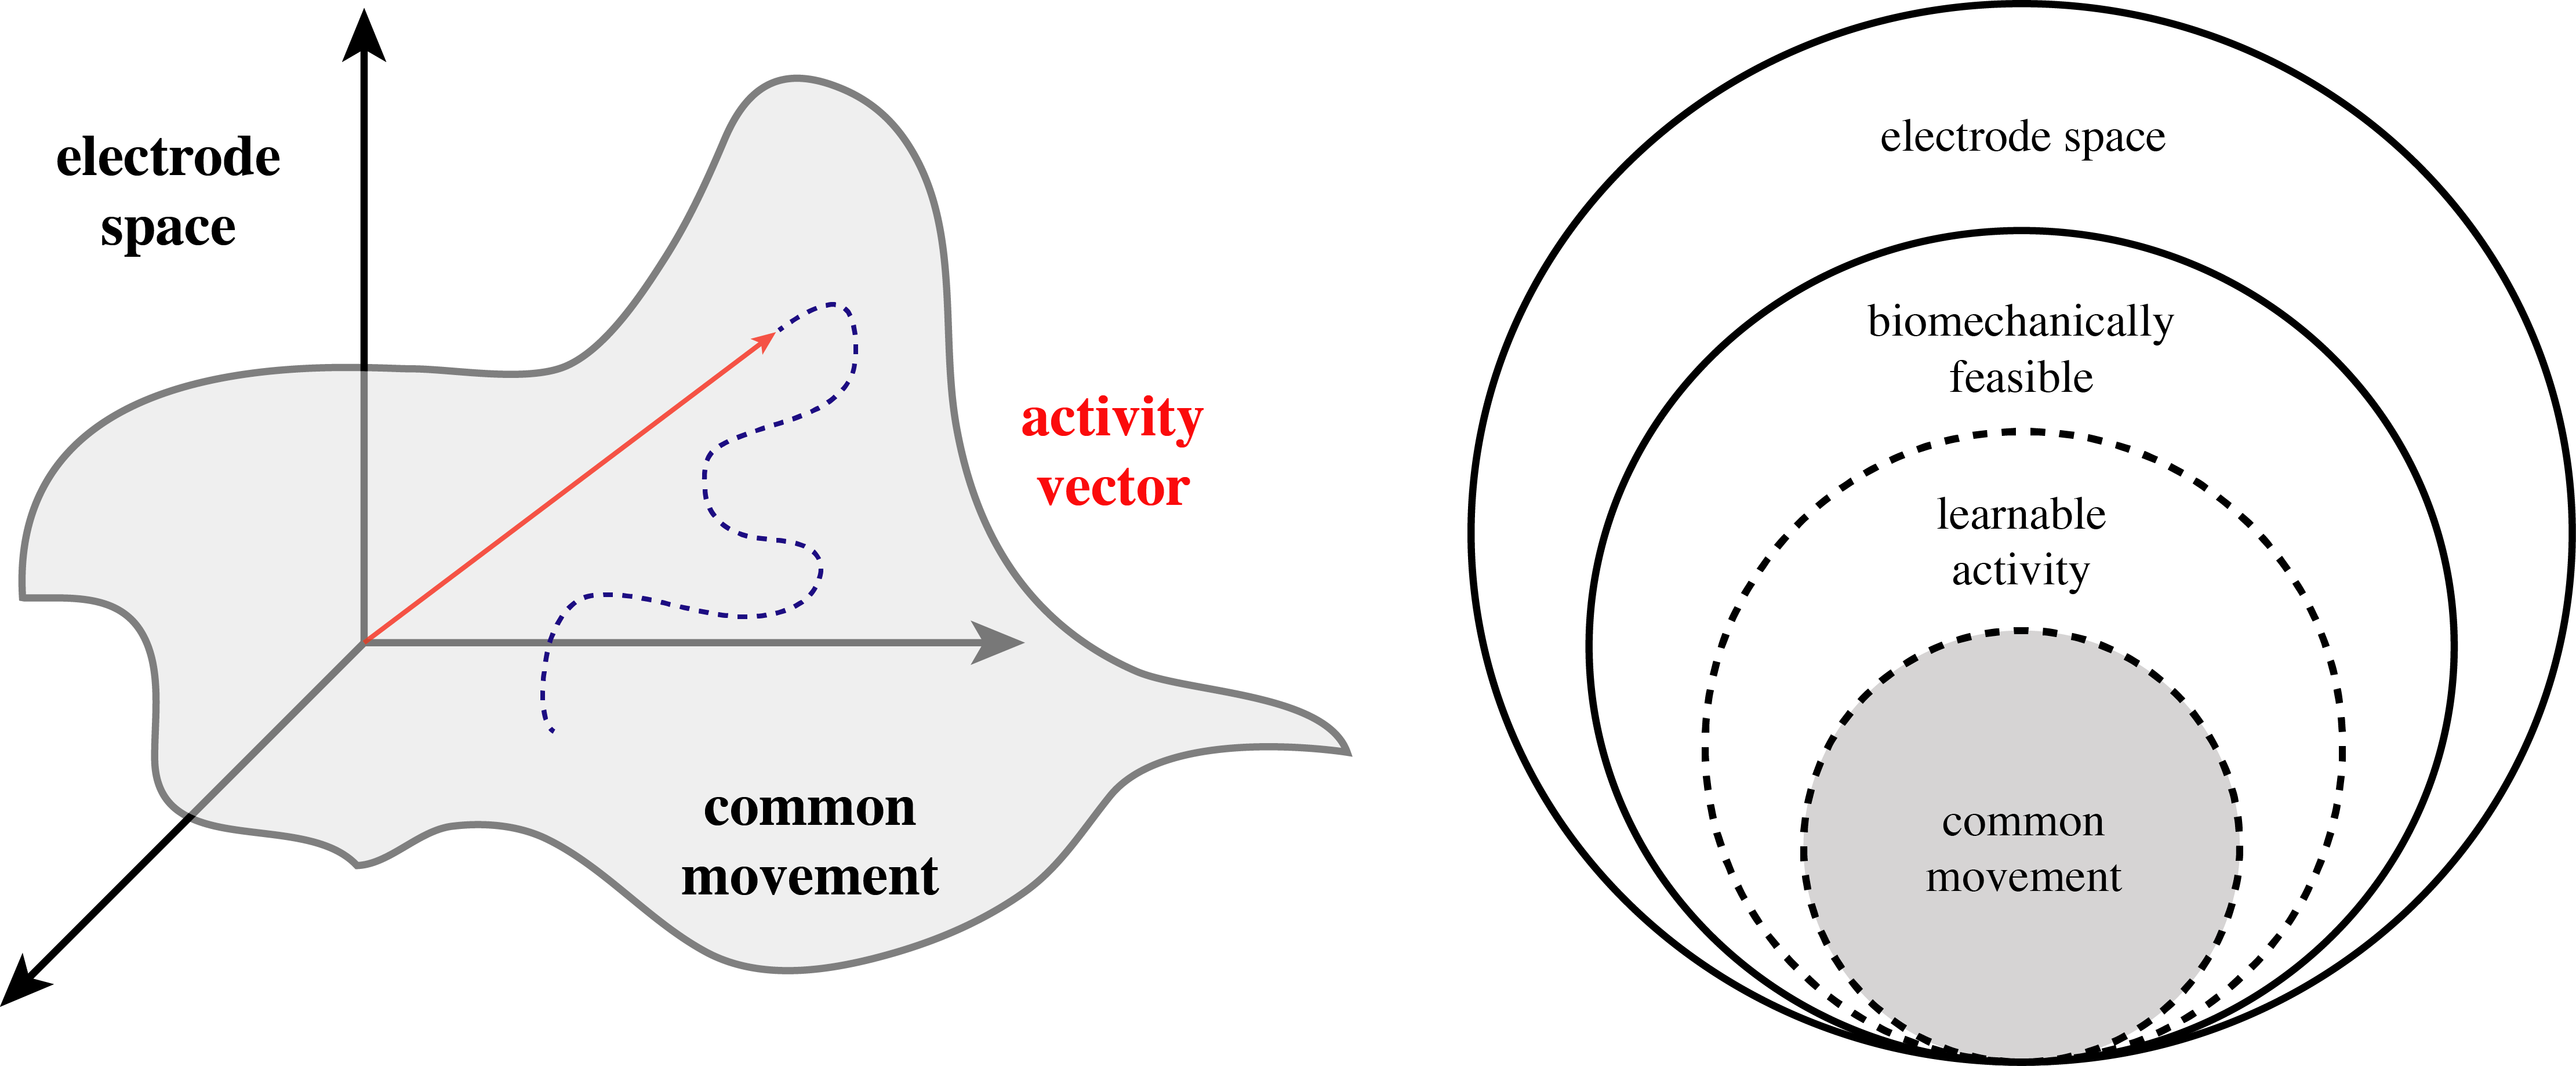
\includegraphics[width=1.0\textwidth]{methods/spaces.pdf}
  \caption[Sketch of the task geometry]{Sketch of the task geometry. Shown in 3-dimensions, simplified from 64, the ambient EMG space denotes all of the possible signals we could capture using our EMG recoding apparatus. The movement manifold depicts the (nonlinear) subspace of the ambient EMG space in which subjects can move, and which we can capture from subjects given constraints such as electrode placement and layering of muscle tissue. A single time point of subjects EMG signal is a vector in the EMG space, and over time these activations trace out trajectories through this space. We project these activations using our decoder, which places the activations onto a 2-dimensional plane, the decoder plane. Targets ``live'' on this plane. Any activity which is nullified through projection onto the decoder plane is within the null space of the decoder. Activity which is not nullified lives in the decoder space.}\label{fig:spaces}
\end{figure}







\section{Recording Setup}\label{sec:setup}

\subsection{Hardware}

Apart from the ``Sessantaquattro'' EMG amplifier acquired from OT Bioelettronica, the hardware was purpose built for this experiment. The amplifier transmits data over WiFi connection with a main data collection machine. Wireless recording enable flexibility in terms of wiring and placement of the accompanying components. A custom printed circuit board was built to provide electronic connection between the amplifier and the 64 monopolar EMG electrodes. The 10mm Ag-AgCl reusable cup electrodes acquired from UniMed UK We used conductive gel acquired from UniMed UK (brand name AC Cream) to provide a conductive interface between skin and electrode. A reference electrode was attached to subjects' ulnar styloid. EMG signals were captured at 2kHz with 24-bit precision. A short example segment of raw data is shown in \Cref{fig:raw_data}. As shown in \Cref{fig:prototype_setup}, several prototypes were made and tested for an electrode arrangement which permitted different size arms, was comfortable for the wearer, and ensured that electrodes remained in contact with the skin. The final design uses an elastic sleeve with the ability to ``snap'' connect electrodes to the sleeve to allow for different sized arms and replacement of electrodes in case of faults. 

During the recording sessions, as shown in \Cref{fig:final_setup}, the subject's arm is enclosed within a metal frame to shield noise as well as to remove the arm from the subject's field of view. The subject's arm is constrained in a foam-filled fixture to encourage isometric contractions. This enables the experiment to me more repeatable over subjects and decreases the likelihood of signal artefacts. 64 electrodes were attached to subjects' arms in a rectangular grid pattern, attempting to cover as much of the forearm musculature as possible. The electrode layout is shown in \Cref{fig:muscle_map} with electrodes denoted blue blue markers.

\subsection{Software}

We employed the versatile Bonsai programming environment\endnote{For more information, please visit the \href{https://bonsai-rx.org/}{Bonsai-RX Homepage.}}, which supports both C\# and Python programming. Bonsai allowed us to seamlessly integrate online data capture from our EMG sensors with the real-time presentation of visual feedback to our study participants. This closed-loop capability was crucial for creating an interactive virtual environment where subjects could perceive and respond to the consequences of their muscle activations in real time. Bonsai is an invaluable tool for neuroscience, and scientific research generally.

The raw EMG data was initially acquired and pre-processed within the Bonsai environment. An example of the raw EMG traces recorded from a representative participant is depicted in \Cref{fig:raw_data}. While Bonsai facilitated the online aspects of our experiment, all subsequent offline analyses were performed using Python.

Our Python code implemented a comprehensive analysis pipeline that handled data filtering, epoch extraction, artifact removal, and feature extraction from the high-dimensional EMG datasets. All of the software, spanning the Bonsai source code for online operations to the custom Python analysis scripts, is openly available to interested researchers upon request. We firmly believe in promoting open science and ensuring the reproducibility of our methods. Sharing this code will allow others to validate, extend or build upon our work.

\begin{figure}[!htb]
\centering
\includegraphics[width=1.0\textwidth]{methods/setup.pdf}
\caption[Experimental setup prototype]{(a) Graphic depicting the closed-loop EMG interface concept in a target task. The multidimensional EMG signal is transformed online through a mapping $F$ from EMG electrode space to a lower dimensional task space, creating an experimentally controllable redundancy problem for the subject. In experiments shown here the task space is two-dimensional, though the EMG interface can be extended to tasks with higher-dimensional inputs. The subject's arm and hand are constrained during the experiment to ensure isometric contractions. (b) First prototype of custom recording hardware consisting of four bands of eight electrodes each, and a spherical hand constraint. Our recordings are 64 channel monopolar recording with reference electrode at the wrist. (c) Example cup-style monopolar recording electrodes, 5mm in diameter. (d) Side view of the recording hardware. Also pictured is the arm restraint frame to ensure isometric contractions. The frame obscures the subject's arm from view and contains adjustable elbow and wrist rests. (d) Recording hardware shown off the arm with wireless amplifier and connection board.}\label{fig:prototype_setup}
\end{figure}

\begin{figure}[!htb]
  \centering
  \begin{minipage}{0.33\textwidth}
    \includegraphics[width=\textwidth]{methods/electrode_assembly.png}
    \subcaption{}
  \end{minipage}%
  \hspace*{5pt}
  \begin{minipage}{0.33\textwidth}
    \includegraphics[width=\textwidth]{methods/electrode_detail.JPG}\\
    \subcaption{}
    \includegraphics[width=\textwidth]{methods/hand_constraint_detail.JPG}
    \subcaption{}
  \end{minipage}%
  \hspace*{5pt}
  \begin{minipage}{0.33\textwidth}
    \includegraphics[width=\textwidth]{methods/hand_constraint_in_box.JPG}\\
    \subcaption{}
    \includegraphics[width=\textwidth]{methods/peter_playing_game.JPG}
    \subcaption{}
  \end{minipage}
  \caption[Final experimental setup]{(a) Final design of the electrode assembly, showing the elastic sleeve with embedded electrodes, and Velcro closure (b) Closeup of the 3D printed electrode hardware to enable ``snap'' connections with the sleeve (c) Hand constraint, 3D printed plastic with medical-grade foam (d) Entire electrode assembly within the recorded enclosure (e) Subject engaged in the natural movement task}\label{fig:final_setup}
\end{figure}

\begin{figure}[!htb]
  \centering
  \includegraphics[width=1.0\textwidth]{methods/muscle_map.pdf}
  \caption[Electrode layout with forearm and hand muscles]{Layout of the forearm muscles showing, in blue, the approximate locations where electrodes were placed on subjects's arms during the experiment.}\label{fig:muscle_map}
\end{figure}

\begin{figure}[!htb]
  \centering
  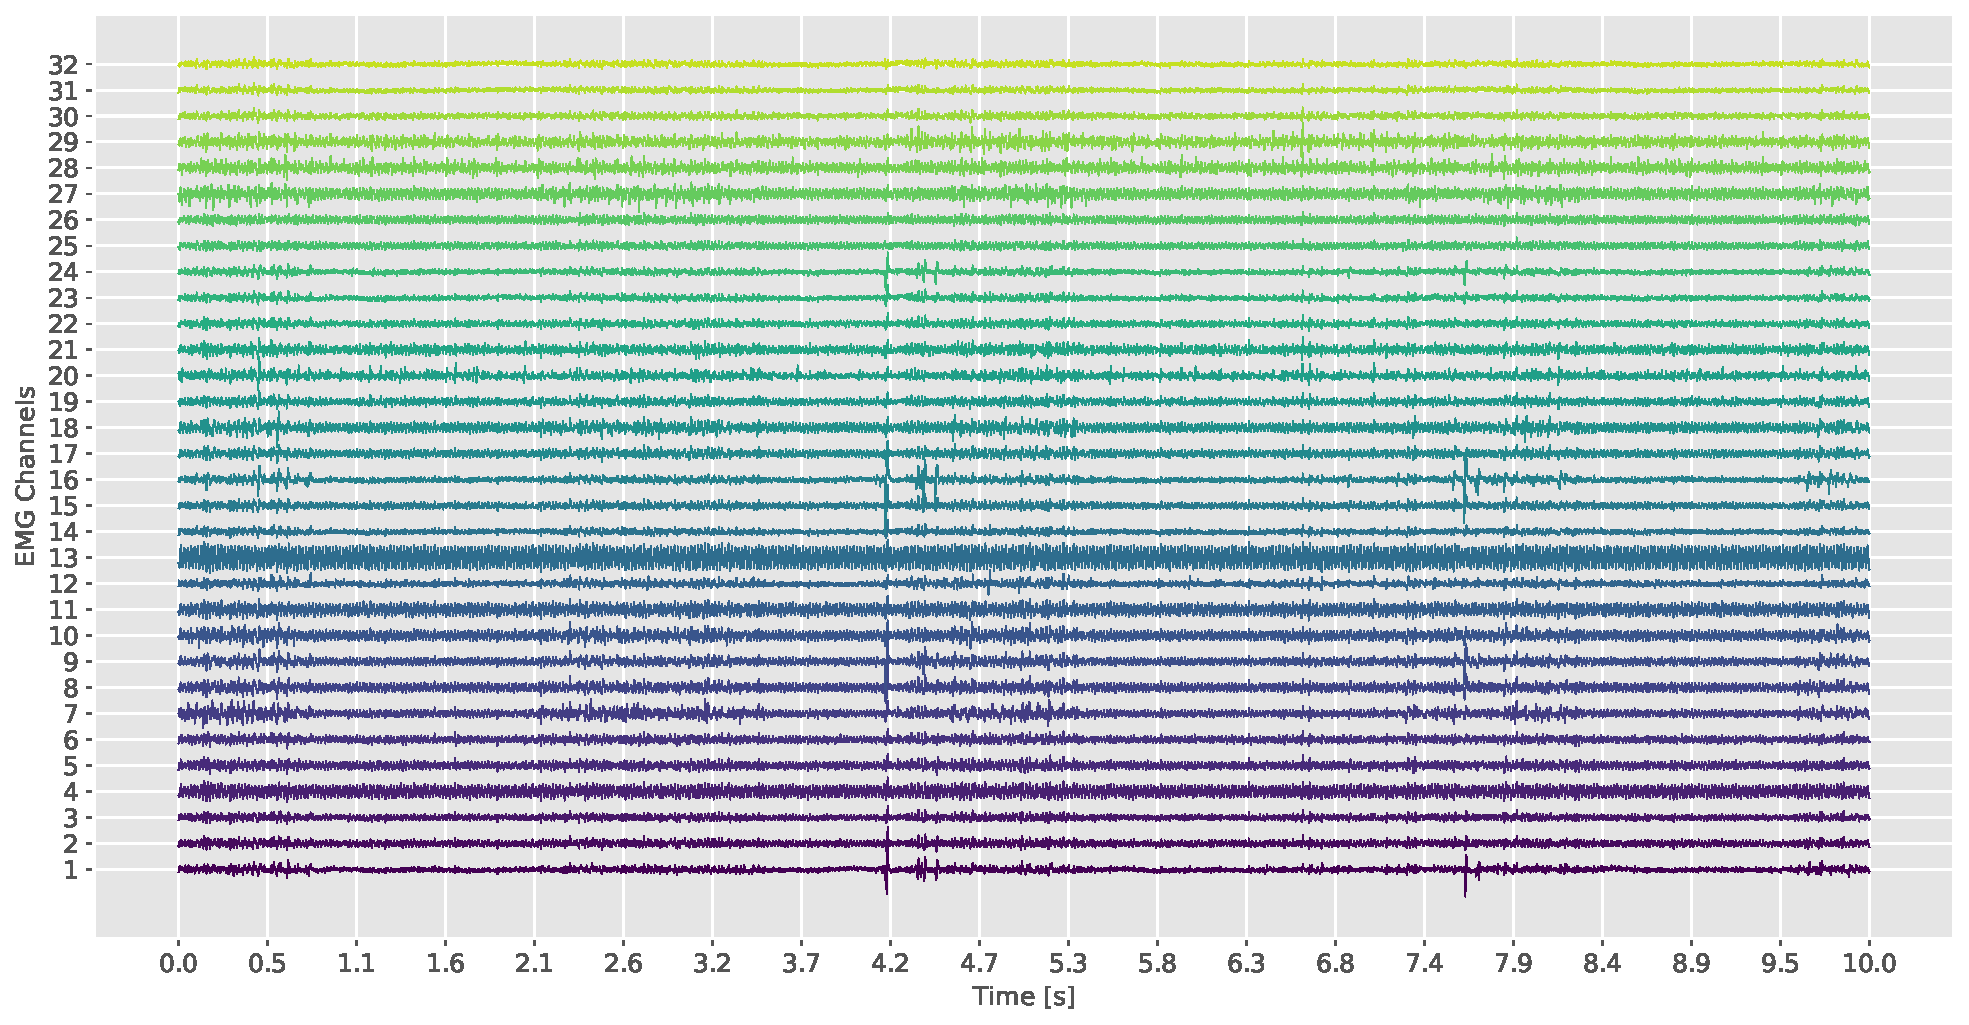
\includegraphics[width=1.0\textwidth]{methods/raw_data.pdf}
  \caption[Example raw EMG data]{10 seconds of raw 64-channel EMG data taken during a finger flexion trial. Note that some channels include some clear sine wave line noise. Putative single motor unit action potentials can be seen on many channels.}\label{fig:raw_data}
\end{figure}







\section{Task Structure}

% The steps of each subject's trial:

% \begin{enumerate}
%   \item There are three parts of each subject's recording session: natural movement, calibration, and the target task
%   \item before beginning:
%   \begin{enumerate}
%     \item 
%     \item enter subject details, consent form sign
%     \item measure arm (at ulnar styloid and 5cm below tip of elbow)
%     \item choose closest sleeve size, erring on the small side, attach electrodes
%     \item apply electrode paste to each electrode
%     \item pre-task form fill-in (with subject metadata)
%     \item clean and prep arm: soap and warm water, hard scrub
%     \item place sleeve 2cm from ulnar styloid
%     \item place arm in enclosure, secure hand and arm using velcro straps
%     \item attach electronic ground wires to enclosure
%     \item test recording: look for obvious signs of noise, electrode liftoff
%     \item if issues found, adjust band, individual electrodes, or wiring
%     \item explain task structure
%   \end{enumerate}
%   \item natural movement task:
%   \begin{enumerate}
%     \item ``You will be asked to perform a series of movements in the following order, \lbrack{read each movement, demonstrating each one}\rbrack. The name of each movement will appear on the screen. When the green dot appears, make this movement and hold it until the green dot disappears. The dot will last for 1 second, with a 1 second break. This will repeat three times for each movement. Try to achieve each movement to the best of your ability. Do not use your maximum force for each movement, aim for approximately 50\% of your maximum.''
%     \item Answer any questions the subject may have about the task, ask if they are ready to begin
%     \item Repeat this task (the series of all movements) twice 
%   \end{enumerate}
%   \item calibration bar task:
%   \begin{enumerate}
%     \item you will be asked to perform an ``exploration and isolation'' task
%     \item you will see 64 vertical bars on your screen, 63 of which are white and one which is red
%     \item your movements cause the bars to change in height on the screen
%     \item your goal on each trial is to attempt, to the best of your ability, to maximize the height of the red bar while minimizing the height of all other bars
%   \end{enumerate}
%   \item fit the target task decoder:
%   \begin{enumerate}
%     \item run nonnegative matrix factorization with 4 components on the filtered calibration data
%     \item visually inspect the modes
%     \item compute the decoder, details in \Cref{sec:decoder_fitting}
%     \item if an error is seen, emg is checked, calibration is repeated
%     \item otherwise store the decoder and move to the target task
%   \end{enumerate}
%   \item target task:
%   \begin{enumerate}
%     \item you will be asked to move a white circular cursor from the center of the screen to a red circular targets using the muscles controlling your hand
%     \item first, you must hold the cursor in the center of the screen for a required time, after which a red target will appear and the trial will begin. for the cursor to remain in the center of the screen, you must fully relax your arm and shoulder
%     \item \lbrack{help the subject practice relaxing their arm, as you can hold tension in your arm and hand without realizing it. give the subject verbal instruction to help them fully relax}\rbrack
%     \item if you fail to hold the cursor in the center at the start of the trial, the trial will time out and you will have three more chances to hold
%     \item each trial you will attempt to hit the target with your cursor. if you are successful, a new trial will begin. if you run out of time, a new trial will begin
%     \item you will attempt to complete 540 trials in total, with short breaks after each group of 180 trials
%     \item after each group, I briefly interview you about any issues as needed
%   \end{enumerate}
%   \item \textbf{TODO} I need to explain the task spaces here more deeply, the kind of paradigm we are aiming to develop... I need a (better) figure that summarizes the linear algebra of the EMG space and the task space! I have \Cref{fig:spaces} now
%   \item Each subject took about 3 hours to complete data collection 
%   \end{enumerate}
%     \item if issues found, adjust band, individual electrodes, or wiring
%     \item explain task structure
%   \end{enumerate}
%   \item natural movement task:
%   \begin{enumerate}
%     \item ``You will be asked to perform a series of movements in the following order, \lbrack{read each movement, demonstrating each one}\rbrack. The name of each movement will appear on the screen. When the green dot appears, make this movement and hold it until the green dot disappears. The dot will last for 1 second, with a 1 second break. This will repeat three times for each movement. Try to achieve each movement to the best of your ability. Do not use your maximum force for each movement, aim for approximately 50\% of your maximum.''
%     \item Answer any questions the subject may have about the task, ask if they are ready to begin
%     \item Repeat this task (the series of all movements) twice 
%   \end{enumerate}
%   \item calibration bar task:
%   \begin{enumerate}
%     \item you will be asked to perform an ``exploration and isolation'' task
%     \item you will see 64 vertical bars on your screen, 63 of which are white and one which is red
%     \item your movements cause the bars to change in height on the screen
%     \item your goal on each trial is to attempt, to the best of your ability, to maximize the height of the red bar while minimizing the height of all other bars
%   \end{enumerate}
%   \item fit the target task decoder:
%   \begin{enumerate}
%     \item run nonnegative matrix factorization with 4 components on the filtered calibration data
%     \item visually inspect the modes
%     \item compute the decoder, details in \Cref{sec:decoder_fitting}
%     \item if an error is seen, emg is checked, calibration is repeated
%     \item otherwise store the decoder and move to the target task
%   \end{enumerate}
%   \item target task:
%   \begin{enumerate}
%     \item you will be asked to move a white circular cursor from the center of the screen to a red circular targets using the muscles controlling your hand
%     \item first, you must hold the cursor in the center of the screen for a required time, after which a red target will appear and the trial will begin. for the cursor to remain in the center of the screen, you must fully relax your arm and shoulder
%     \item \lbrack{help the subject practice relaxing their arm, as you can hold tension in your arm and hand without realizing it. give the subject verbal instruction to help them fully relax}\rbrack
%     \item if you fail to hold the cursor in the center at the start of the trial, the trial will time out and you will have three more chances to hold
%     \item each trial you will attempt to hit the target with your cursor. if you are successful, a new trial will begin. if you run out of time, a new trial will begin
%     \item you will attempt to complete 540 trials in total, with short breaks after each group of 180 trials
%     \item after each group, I briefly interview you about any issues as needed
%   \end{enumerate}
%   \item \textbf{TODO} I need to explain the task spaces here more deeply, the kind of paradigm we are aiming to develop... I need a (better) figure that summarizes the linear algebra of the EMG space and the task space! I have \Cref{fig:spaces} now
%   \item Each subject took about 3 hours to complete data collection 
%   \end{enumerate}
%     \item if issues found, adjust band, individual electrodes, or wiring
%     \item explain task structure
%   \end{enumerate}
%   \item natural movement task:
%   \begin{enumerate}
%     \item ``You will be asked to perform a series of movements in the following order, \lbrack{read each movement, demonstrating each one}\rbrack. The name of each movement will appear on the screen. When the green dot appears, make this movement and hold it until the green dot disappears. The dot will last for 1 second, with a 1 second break. This will repeat three times for each movement. Try to achieve each movement to the best of your ability. Do not use your maximum force for each movement, aim for approximately 50\% of your maximum.''
%     \item Answer any questions the subject may have about the task, ask if they are ready to begin
%     \item Repeat this task (the series of all movements) twice 
%   \end{enumerate}
%   \item calibration bar task:
%   \begin{enumerate}
%     \item you will be asked to perform an ``exploration and isolation'' task
%     \item you will see 64 vertical bars on your screen, 63 of which are white and one which is red
%     \item your movements cause the bars to change in height on the screen
%     \item your goal on each trial is to attempt, to the best of your ability, to maximize the height of the red bar while minimizing the height of all other bars
%   \end{enumerate}
%   \item fit the target task decoder:
%   \begin{enumerate}
%     \item run nonnegative matrix factorization with 4 components on the filtered calibration data
%     \item visually inspect the modes
%     \item compute the decoder, details in \Cref{sec:decoder_fitting}
%     \item if an error is seen, emg is checked, calibration is repeated
%     \item otherwise store the decoder and move to the target task
%   \end{enumerate}
%   \item target task:
%   \begin{enumerate}
%     \item you will be asked to move a white circular cursor from the center of the screen to a red circular targets using the muscles controlling your hand
%     \item first, you must hold the cursor in the center of the screen for a required time, after which a red target will appear and the trial will begin. for the cursor to remain in the center of the screen, you must fully relax your arm and shoulder
%     \item \lbrack{help the subject practice relaxing their arm, as you can hold tension in your arm and hand without realizing it. give the subject verbal instruction to help them fully relax}\rbrack
%     \item if you fail to hold the cursor in the center at the start of the trial, the trial will time out and you will have three more chances to hold
%     \item each trial you will attempt to hit the target with your cursor. if you are successful, a new trial will begin. if you run out of time, a new trial will begin
%     \item you will attempt to complete 540 trials in total, with short breaks after each group of 180 trials
%     \item after each group, I briefly interview you about any issues as needed
%   \end{enumerate}
%   \item \textbf{TODO} I need to explain the task spaces here more deeply, the kind of paradigm we are aiming to develop... I need a (better) figure that summarizes the linear algebra of the EMG space and the task space! I have \Cref{fig:spaces} now
%   \item Each subject took about 3 hours to complete data collection 
%   \end{enumerate}


Each subject's recording session consisted of three main parts: natural movement, calibration, and the target task. Prior to beginning, the following preparatory steps were taken:
%
\begin{enumerate}
  \item The subject's details were entered, and they signed a consent form.
  \item The subject's arm was measured at the ulnar styloid and 5cm below the tip of the elbow.
  \item The closest sleeve size was chosen, erring on the small side, and electrodes were attached.
  \item Electrode paste was applied to each electrode.
  \item The subject completed a pre-task form with their metadata.
  \item The subject's arm was cleaned and prepped by scrubbing with soap and warm water.
  \item The sleeve was placed 2cm from the ulnar styloid.
  \item The subject's arm was secured in the enclosure using Velcro straps, with the hand also secured.
  \item Electronic ground wires were attached to the enclosure.
  \item A test recording was performed to check for obvious signs of noise or electrode liftoff.
  \item If issues were found, the band, individual electrodes, or wiring were adjusted.
  \item The task structure was explained to the subject.
\end{enumerate}
%
The natural movement task proceeded as follows:
%
\begin{enumerate}
  \item The subject was instructed to perform a series of movements in a specific order, with each movement being demonstrated.
  \item The name of each movement would appear on the screen, followed by a green dot. When the dot appeared, the subject would make that movement and hold it until the dot disappeared (1 second), with a 1-second break between repetitions.
  \item Each movement was repeated three times, with the subject aiming for approximately 50\% of their maximum force.
  Any questions from the subject were addressed, and they were asked if they were ready to begin.
  \item The series of movements was repeated twice.
\end{enumerate}
%
Next, the calibration bar task was performed:
%
\begin{enumerate}
  \item The subject was asked to perform an ``exploration and isolation'' task.
  \item They would see 64 vertical bars on the screen, 63 white and one red.
  \item Their movements would cause the bars to change in height.
  \item The goal for each trial was to maximize the height of the red bar while minimizing the height of all other bars.
\end{enumerate}
%
This calibration task was designed to push subjects towards decorrelating their EMG channels to the best of their ability. This would, in theory, produce a dataset depicting the boundaries or limits of the EMG manifold, providing a useful training set for subject-specific decoders. We took inspiration in this design from the extraction of features from spontaneous activity and passive viewing used in cortical BMI experiments to generate ``intuitive'' mappings\cite{clancySensoryRepresentationCausally2019a,sadtlerNeuralConstraintsLearning2014}.
%
Next, the target task decoder was fitted:
%
\begin{enumerate}
  \item Nonnegative matrix factorization with 4 components was run on the filtered calibration data.
  \item The modes were visually inspected.
  \item The decoder was computed (details in \Cref{sec:decoder_fitting}).
  \item If an error was seen, the EMG was checked, and the calibration was repeated.
  \item Otherwise, the decoder was stored, and the subject proceeded to the target task.
\end{enumerate}
%
The target task proceeded as follows:
%
\begin{enumerate}
  \item The subject was asked to move a white circular cursor from the center of the screen to a red circular target using the muscles controlling their hand.
  \item First, the subject had to hold the cursor in the center for a required time, after which a red target would appear, and the trial would begin. To hold the cursor in the center, the subject had to fully relax their arm and shoulder.
  \item The subject was given verbal instructions and practice to help them fully relax their arm.
  If the subject failed to hold the cursor in the center at the start of the trial, the trial would time out, and they would have three more chances to hold.
  \item The subject attempted to hit the target with the cursor. If successful, a new trial would begin. If they ran out of time, a new trial would begin.
  \item The subject attempted to complete 540 trials in total, with short breaks after each group of 180 trials.
  \item After each group, the subject was briefly interviewed about any issues.
\end{enumerate}
%
It took on average 3 hours for each subject to complete the data collection session.

\begin{figure}[!htb]
  \centering
  \includegraphics[width=1.0\textwidth]{methods/task_structure.pdf}
  \caption[Task structure for each subject]{Task structure for each subject over the course of a single session.}\label{fig:task_structure}
\end{figure}
  






\subsection{Decoder Fitting}\label{sec:decoder_fitting}

EMG-to-task decoders are computed using a calibration dataset collected before the ``center hold, reach out'' task. 4 ``modes'' of EMG activity are extracted from the dataset using non-negative matrix factorization. These 4 modes are then subtracted in pairs to yield the two 64-dimensional EMG-to-force mappings, shown in \Cref{fig:example_decoder}. 

The EMG signal is inherently nonnegative, as it represents the electrical activity of muscles which cannot have negative activations. Our goal is to extract representative modes from the calibration data; directions in the high-dimensional EMG space that effectively capture the salient statistics of the dataset. We are not primarily concerned with overfitting in this step, as our objective is simply to create a two-dimensional plane within the EMG space where the likelihood that each subject's activity manifold ``covers'' or has access to the domain of the task space is high.

To achieve this, we employed Nonnegative Matrix Factorization (NMF), an unsupervised decomposition technique particularly well-suited for nonnegative data like EMG signals. NMF is a matrix factorization algorithm that approximates a nonnegative matrix $X$ as the product of two low-rank nonnegative factor matrices: $X\approx WH$. Here, $X$ represents the $m\times{n}$ data matrix of EMG recordings, $W$ is an $m\times{k}$ matrix containing k basis vectors that comprise a linear subspace, and H is the corresponding $n\times{k}$ matrix of nonnegative coefficients that encode the representation of $X$ in the basis defined by $W$. Mathematically, nonnegative matrix factorization (NMF) is the solution to the following optimization problem:

\begin{align}
  \min{||X - WH||^{2}}
\end{align}

where $X$ is our calibration EMG data, concatenated along samples with shape $(c\times{n})$ where $N$ is the number of samples and $C$ is the number of electrode channels, fixed at 64. The objective assumes that this EMG data can be accurately reconstructed by a dot product between $W$, a $c\times{m}$ matrix which holds $m$ ``modes'', and $H$, an $m\times{n}$ matrix which holds $n$ ``activations''. For our purposes we choose \textit{a priori} to fit 4 modes, one for each cardinal direction: up, down, left, and right. The NMF process can be thought of as extracting, or inferring, an $m$-dimensional linear latent space (an $m$ dimensional plane) within the 64-dimensional EMG space which ``generates'' the data. This $m$ dimensional plane, in order to reconstruct the full 64D signal, must capture the salient features of the original data.

The key benefit of NMF over other techniques like Principal Component Analysis is that the extracted basis vectors (columns of $W$) are constrained to be fully nonnegative and not required to be orthogonal, which makes them interpretable as ``parts'' or ``components'' that are additive and combined by the nonnegative coefficients in $H$ to represent the original data. This additive parts-based representation has been shown to capture intuitive notions of objects or semantic features in data like images, text, and neural signals\cite{leeLearningPartsObjects1999a,eggertSparseCodingNMF2004}. A visual comparison of NMF and PCA is shown in \Cref{fig:nmf_v_pca}.

In our case, the columns of $W$ corresponded to putative muscle synergies or coordinated activations extracted directly from the calibration EMG data in an unsupervised manner. By projecting this data into the 2D subspace defined by the top two basis vectors, we obtained a compact representation that still encoded rich structure present in the high-dimensional recordings in an intuitive format designed to respect the nonnegative nature of the signal. This 2D embedding formed the basis for our subsequent online EMG-to-cursor mapping used in the main target task.

\begin{figure}[!htb]
  \centering
  \includegraphics[width=1.0\textwidth]{methods/NMF_PCA_comparison.pdf}
  \caption[Comparison of NMF and PCA]{Comparison of NMF and PCA. The leftmost plot shows a random sample fro a mixture of two 2D Gaussians (black). PCA on this data returns a simple rotation of the data aligned with the directions of maximum variance (blue arrows). The middle plot shows this data exponentiated, or log-normal. NMF is run on this data with two components and the directions which are found to maximally reconstruct this data are show (purple arrows). In the rightmost plot, we log-transform this exponentiated data (black) as well as the NMF axes (orange arrows). We also normalize these transformed axes. Thus we have a nonnegative basis for the data via NMF in both the original and log-normal spaces which reflect the dominant modes of the data, as used to generate our task decoders. This highlights the key difference between PCA and NMF\: PCA is concerned with data variance, while NMF is a ``best fit'' (up to an error tolerance) of the data's modes and does not have an immediate notion of ``explained variance''. PCA reconstructs variance, NMF reconstructs the data itself using additive components. In our task, NMF is used on the log-normal data to find modes. If comparisons are made between datasets, PCA and NMF subspaces should be compared like for like; for which this demonstration provides geometric intuition.}\label{fig:nmf_v_pca}
\end{figure}

Each NMF mode is made of up weights for each EMG channel. Once fit to a dataset, each mode can be thought of as a linear filter for each filtered EMG sample, within the original dataset or a new sample. Each filtered sample is ``projected onto'' (the dot product is taken with) each mode. Thus, each 64-dimensional EMG sample $x$ (a point in 64D space) isz reduced to a vector $h$ in a 4D latent space:

\begin{align}
  X &= W\cdot{H} \\
  W^{-1}\cdot{X} &= {H} \\
  h &= W^{-1}\cdot{x}.
\end{align}

This assumes that we can compute the inverse of $W$ which in our case is rectangular. We use the Moore-Penrose pseudoinverse in place of the full inverse. Since two pairs of four modes we extract via NMF correspond to opposite directions and the mapping is linear, we subtract each pair of modes to produce a $2\times{64}$ dimensional mapping

\begin{align}
  D &= \lbrack w_1 - w_2, w_4 - w_3 \rbrack.
\end{align}

This mapping, the difference between pairs of pseudoinverse modes, is what we term the \textit{decoder}. An example of a subject's decoder is shown in \Cref{fig:example_decoder}.

% \begin{itemize}
%   \item \textbf{TODO} Show that we can run NMF on the second calibration dataset and compare – does similarity here correlate with performance?
%   \item Note that these differences in the 4D space lead to a plane through the origin not perpendicular but in the plane of the two differences-- so the decoder plane is the plane spanned by the pairs which are subtracted?
%   \item appropriately relevant to the manifold, but also arbitrary?
% \end{itemize}

\begin{figure}[!htb]
  \centering
  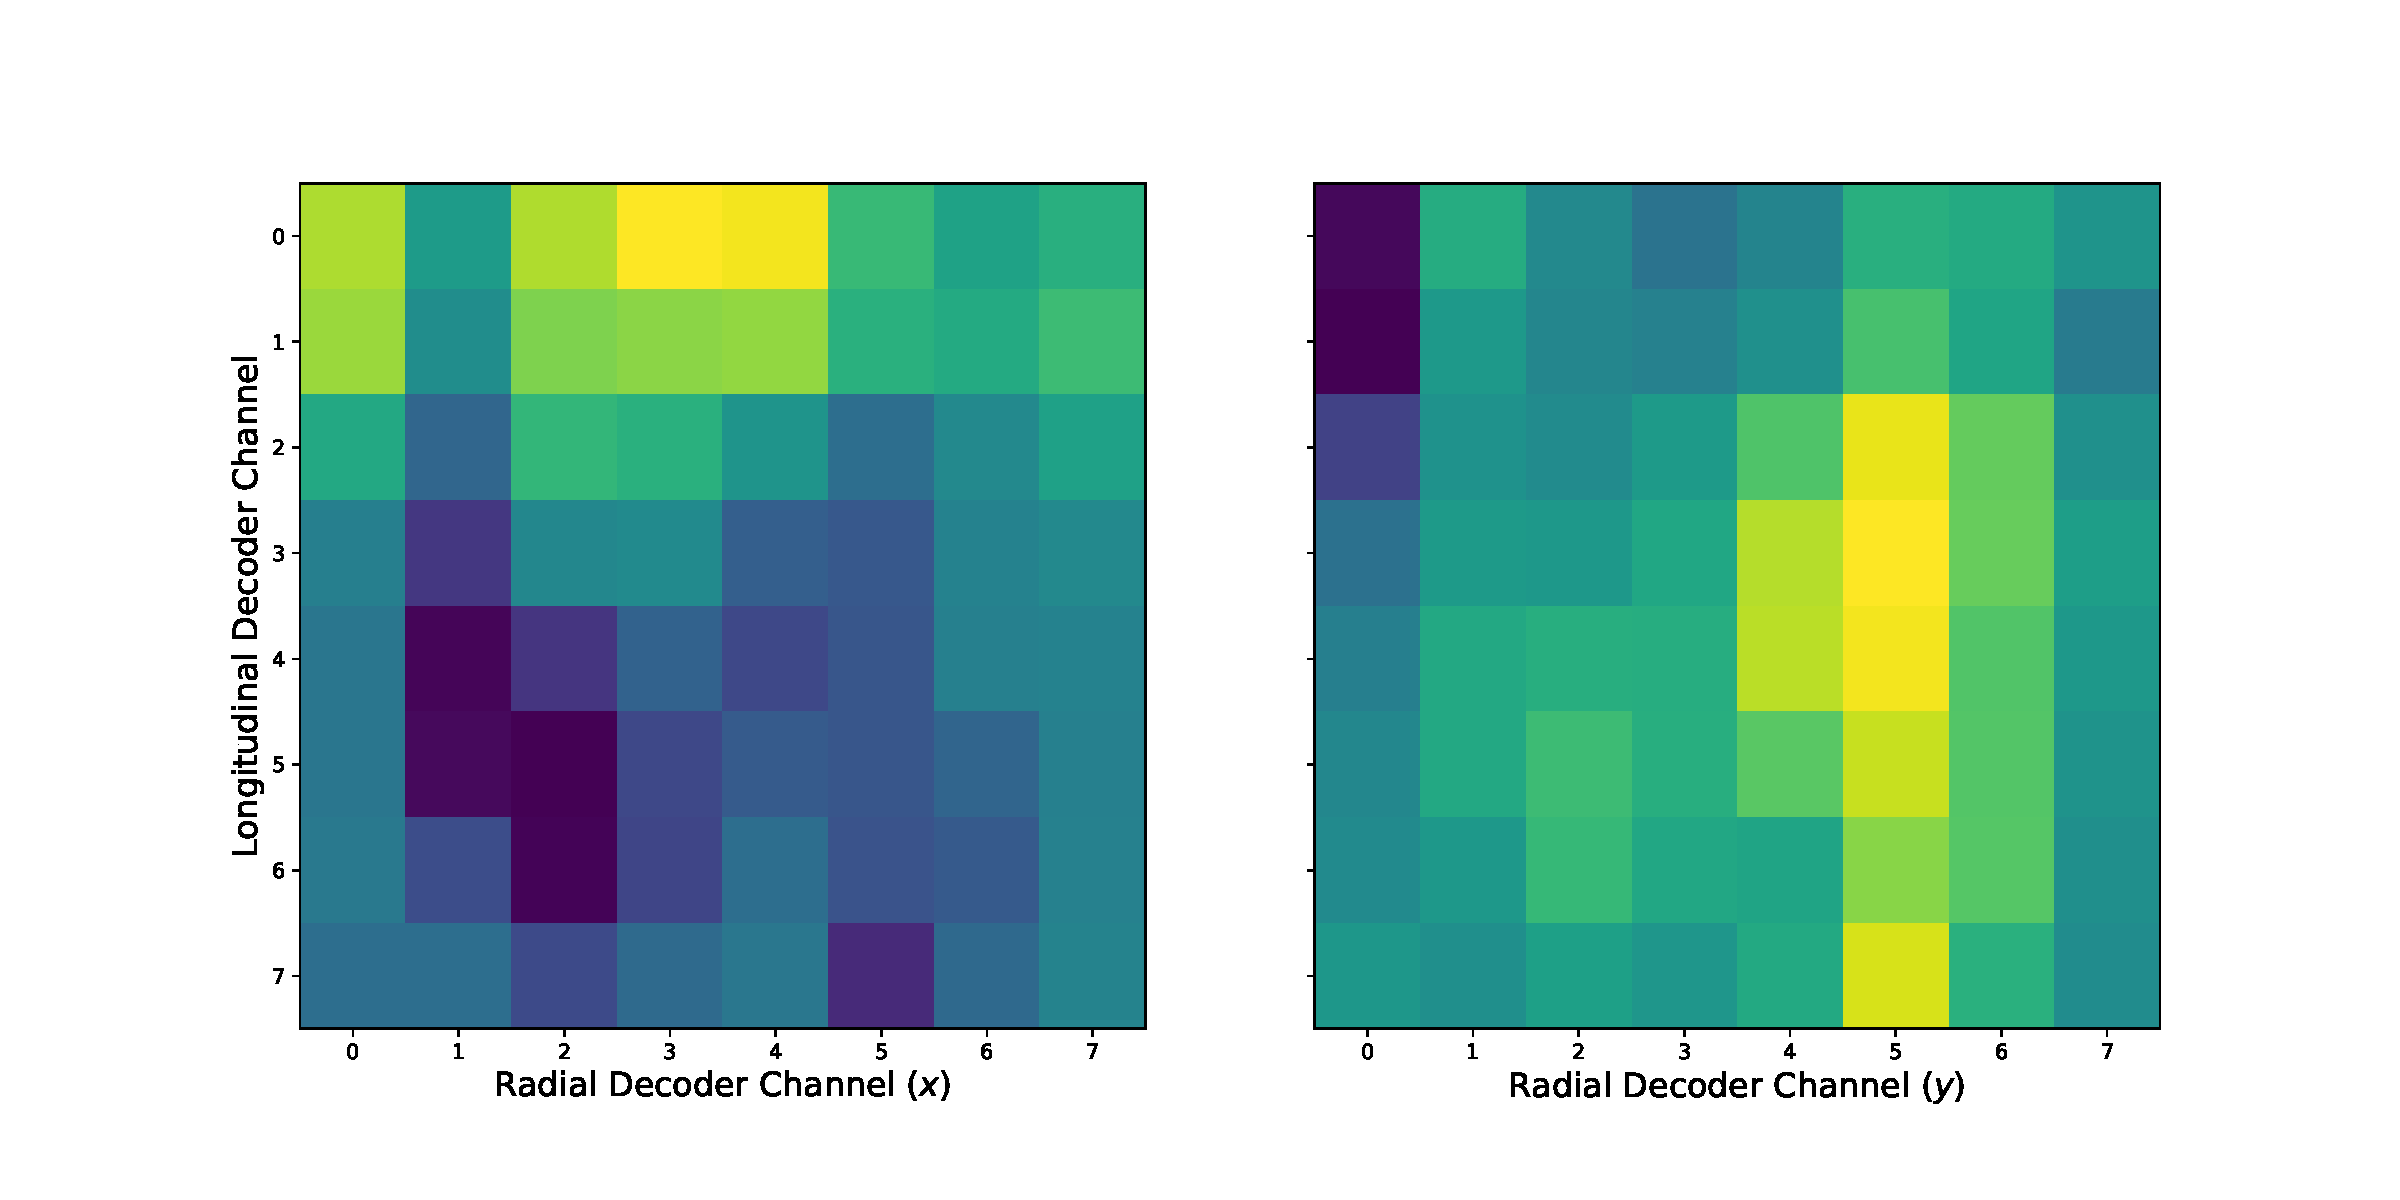
\includegraphics[width=0.7\textwidth]{methods/example_decoder.pdf}
  \caption[Example subject decoder]{Example EMG-to-cursor decoders from a single subject. The target task works by mapping 64 channels of EMG activity from subjects' forearms to 2-dimensional cursor position, a component acting in the $x$ and $y$ directions within the task's linear dynamics. Depicted here are the two 64-dimensional ``decoders'' arranged as the EMG electrodes were arranged on subjects' arms (along the arm, longitudinally, and around the arm, radially). The left plot shows the $x$ cursor decoder mode, with $y$ on the right.}\label{fig:example_decoder}
\end{figure}






% \section{Offline Data Processing}

% \subsection{Is the Decoder Repeatable? \lbrack{Incomplete}\rbrack}

% \begin{itemize} 
%   \item We used NMF to produce decoders from one of the calibration task datasets. 
%   \item If we run NMF on the second calibration task dataset and compare the results to what was used in the task, are the results similar? This would confirm that the EMG space was adequately captured. 
%   \item We can define a distance metric between the two decoders and test if this correlates with performance. Differences in the decoders implies that our experimental decoder did not capture the EMG space adequately enough to provide a reasonable learning challenge.
%   \item \textbf{Hypothesis}: we will see similar results from the second NMF run, which will reject the hypothesis that our decoder does not well-represent subjects' EMG movement space.
%   \item \textbf{Hypothesis}: inter-decoder distance within subjects will correlate negatively with performance (different decoders, less performant). This implies that the decoder's capturing of whole EMG space, opposed to a subspace, enables subjects to perform better on the task. We expect a crossover point here– you want an EMG search space large enough to encompass the task itself, but small enough not to provide too great of a search task for subjects.
% \end{itemize}

% \subsection{Is the Calibration Task Successful? \lbrack{Incomplete}\rbrack}

% \begin{itemize}
%   \item Compare calibration to movement in terms of variance, rank, some metric of dispersion in EMG space. \textbf{How uniformly can subjects reach their EMG space? E.g. compared to a gaussian/uniform with the same statistics?} The calibration task defines the decoder, and thus it is worth confirming that it is successful in encouraging subjects to explore their EMG space. We can compare their activity to the natural movement datasets as a baseline.
%   \item Hypothesis: Variance in the calibration datasets is higher than in the natural movement dataset, even taking all natural movements together. This implies that the calibration dataset encourages exploration of a wider EMG space than that of natural movement.
% \end{itemize}





\subsection{Offline Preprocessing}

A significant portion of the recorded EMG signal corresponds to periods when the subjects are at rest, with minimal muscle activations. To effectively analyze and interpret the data, it is crucial to define and capture the ``active'' parts of the EMG signal, where subjects are engaged in purposeful movements. We base our approach to identifying active segments on the spatial (channel-wise) 2-norm of the EMG signal.

The distribution of spatial norms in EMG data is known to exhibit non-Gaussian characteristics, which is also evident in our dataset\cite{nazarpourNoteProbabilityDistribution2013a,sangerBayesianFilteringMyoelectric2007}. Example histograms illustrating the apparent log-normality of EMG spatial norms are shown in \Cref{fig:log_hist}. To extract the active segments of the EMG signal, we employ the following activity filter:

\begin{enumerate}
  \item First, we compute the 2-norm of the EMG samples across channels at each time point. We then apply a log transformation to this norm, as the log-normal distribution is amenable to thresholding based on the second moment in the log domain. 
  \item Next, we identify samples whose log-transformed norms fall below a threshold based on the mean and standard deviation of the log-norm distribution. For the natural movement and calibration data, we filter out samples with log-norms below half a standard deviation below the mean. For the trial data, we filter out samples below the mean log-norm. While this may appear to be a stringent filter, the log transformation ensures that we reliably remove low-activation samples, effectively extracting moments when subjects are producing goal-oriented movements.
  \item Additionally, we reject outliers by discarding samples whose log-norms fall outside the 1st and 99.9th percentiles of the distribution. This step helps to mitigate the influence of potential artifacts or extreme values that may arise from various sources, such as electrode noise or motion artifacts.
\end{enumerate}

The result of this activity filtering process is illustrated in \Cref{fig:activity_filter}, where the active segments of the EMG signal are highlighted and retained for further analysis, while the periods of inactivity or low muscle activations are effectively removed. By employing this activity filter, we can focus our analyses on the most relevant and informative portions of the EMG data, where subjects are actively engaged in the experimental tasks and producing meaningful muscle activations. This approach allows us to better characterize and interpret the neural strategies and patterns underlying the observed movements and behaviors.

% for movement and calibration data
% log_norm = np.log(np.linalg.norm(signal,axis=1))
% mean_log_norm = np.mean(log_norm)
% std_log_norm = np.std(log_norm)
% # assuming large samples and rv being log-normal, this is roughly the 30th percentile
% mask = log_norm > (mean_log_norm - 0.5*std_log_norm)

% for trial data:
% log_norm = np.log(np.linalg.norm(signal,axis=1))
% mean_log_norm = np.mean(log_norm)
% std_log_norm = np.std(log_norm)
% # assuming large samples and rv being log-normal, this is roughly the 30th percentile
% mask = log_norm > (mean_log_norm - 0.0*std_log_norm)

% cutoffs for all data:
% samples = analysis.remove_nan_rows(subject_stack.transpose(0,1,3,2).reshape(-1,64))
% lognorms = np.log(np.linalg.norm(samples,axis=1))
% return (np.percentile(lognorms,1), np.percentile(lognorms,99.9))
% movement and calibration: 99.5
% trial: 99.9

\begin{figure}[!htb]
  \begin{minipage}[b]{0.8\linewidth}
    \centering
    \includegraphics[width=\textwidth]{methods/log_hist_movement.pdf}
    \subcaption{}
    \vspace{4ex}
  \end{minipage}\\%
  \begin{minipage}[b]{0.8\linewidth}
    \centering
    \includegraphics[width=\textwidth]{methods/log_hist_calibration.pdf}
    \subcaption{}
    \vspace{4ex}
  \end{minipage}\\%
  \begin{minipage}[b]{0.8\linewidth}
    \centering
    \includegraphics[width=\textwidth]{methods/log_hist_trial.pdf}
    \subcaption{}
    \vspace{4ex}
  \end{minipage}
  \caption[Log transforming EMG]{Application of the activity filter to raw EMG data from a representative subject during the target task. We plot histograms of the spatial (channel-wise) 2-norms of the EMG (left column) at each time point and the log-transformation of these samples (right column) for (a) a representative subject's natural movement task, (b) calibration task, and (c) target task. The original EMG data is plotted in grey, with the active samples shown in blue. Vertical lines show statistics of the two histograms as denoted in the figure legend: green for medians, blue for means. Black vertical lines denote the outlier bounds.}\label{fig:log_hist}
\end{figure}

% \begin{figure}[!htb]
%   \centering
%   \includegraphics[width=1.0\textwidth]{methods/activity_filter.pdf}
%   \caption[Activity filter example trial]{Activity filter!}\label{fig:activity_filter}
% \end{figure}

\begin{figure}[!htb]
  \begin{minipage}[b]{0.6\linewidth}
    \centering
    \includegraphics[width=\textwidth]{methods/activity_filter_good_trial.pdf}
    \subcaption{}
    \vspace{4ex}
  \end{minipage}%%
  \begin{minipage}[b]{0.4\linewidth}
    \centering
    \includegraphics[width=\textwidth]{methods/trajectory_filter_good_trial.pdf}
    \subcaption{}
    \vspace{4ex}
  \end{minipage}\\%
  \begin{minipage}[b]{0.6\linewidth}
    \centering
    \includegraphics[width=\textwidth]{methods/activity_filter_long_trial.pdf}
    \subcaption{}
    \vspace{4ex}
  \end{minipage}%%
  \begin{minipage}[b]{0.4\linewidth}
    \centering
    \includegraphics[width=\textwidth]{methods/trajectory_filter_long_trial.pdf}
    \subcaption{}
    \vspace{4ex}
  \end{minipage}
  \caption[Activity filter for EMG and trajectories]{Application of the activity filter to EMG data (left column) and cursor trajectories in the 2D task space (right column) for a successful trial (top row) and an unsuccessful long trial (bottom row) from the target task. The EMG panels show the raw data across channels (gray), the channel-wise spatial norms (red), and the filtered active samples (green). The trajectory panels depict the cursor paths toward the target, with periods of inactivity (red) removed based on the EMG activity filter.}\label{fig:activity_filter}
\end{figure}





\cleardoublepage\printendnotes%
\ifSubfilesClassLoaded{%
    \newpage%
    \bibliography{../bib/bibliography}%
}{}%
\end{document}